\def\stitle{\theexercise\ - Anweisungen 2}
\section{\stitle}
\begin{frame}[t]%
    \frametitle{\stitle}
\medskip

Gegeben sei der folgende Ausschnitt eines Java-Programms.
\lstinputlisting[style=JAVAlines]{anweis-2/Anweis2.java}

\begin{itemize}
\item[(a)] Welcher Buchstabe wird auf dem Bildschirm ausgegeben, falls \code{i} den Wert $1$, $2$, $3$ bzw. $4$ besitzt?
\item[(b)] Realisieren Sie diesen Programmausschnitt mit einer \code{switch}-Anweisung.
\end{itemize}
\end{frame}


\begin{frame}[fragile]%
 \frametitle{a) Strukturprogramm mit Java-Editor}%

\begin{center}
\lstinputlisting[style=JAVAlines]{anweis-2/Anweis2_snippet.java}
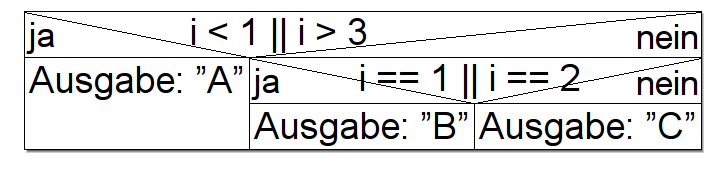
\includegraphics[width=1\textwidth]{anweis-2/Bilder/Struktogramm_a}
\end{center}
\end{frame}


\begin{frame}[fragile]%
 \frametitle{b) Implementierung als \code{switch}-Anweisung}%

\begin{center}
\begin{minipage}{0.7\textwidth}
\begin{lstlisting}[style=JAVA]
switch ( i ) {
  case 1:
  case 2:
    System.out.println("B");
    break;
  case 3:
    System.out.println("C");
    break;
  default:
    System.out.println("A");
}
\end{lstlisting}

\end{minipage}

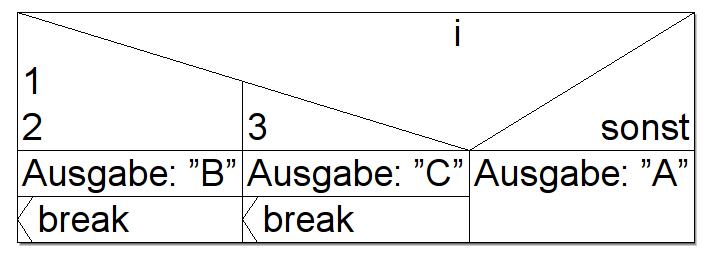
\includegraphics[width=0.6\textwidth]{anweis-2/Bilder/Struktogramm_b}
\end{center}

\end{frame}
